\renewcommand*{\arraystretch}{1.1}

\subsection*{BI / read / 5}
\label{section:bi-read-05}

\noindent\begin{tabularx}{\queryCardWidth}{|>{\queryPropertyCell}p{\queryPropertyCellWidth}|X|}
	\hline
	query & BI / read / 5 \\ \hline
%
	title & Top posters in a country
 \\ \hline
%
	pattern & \hfill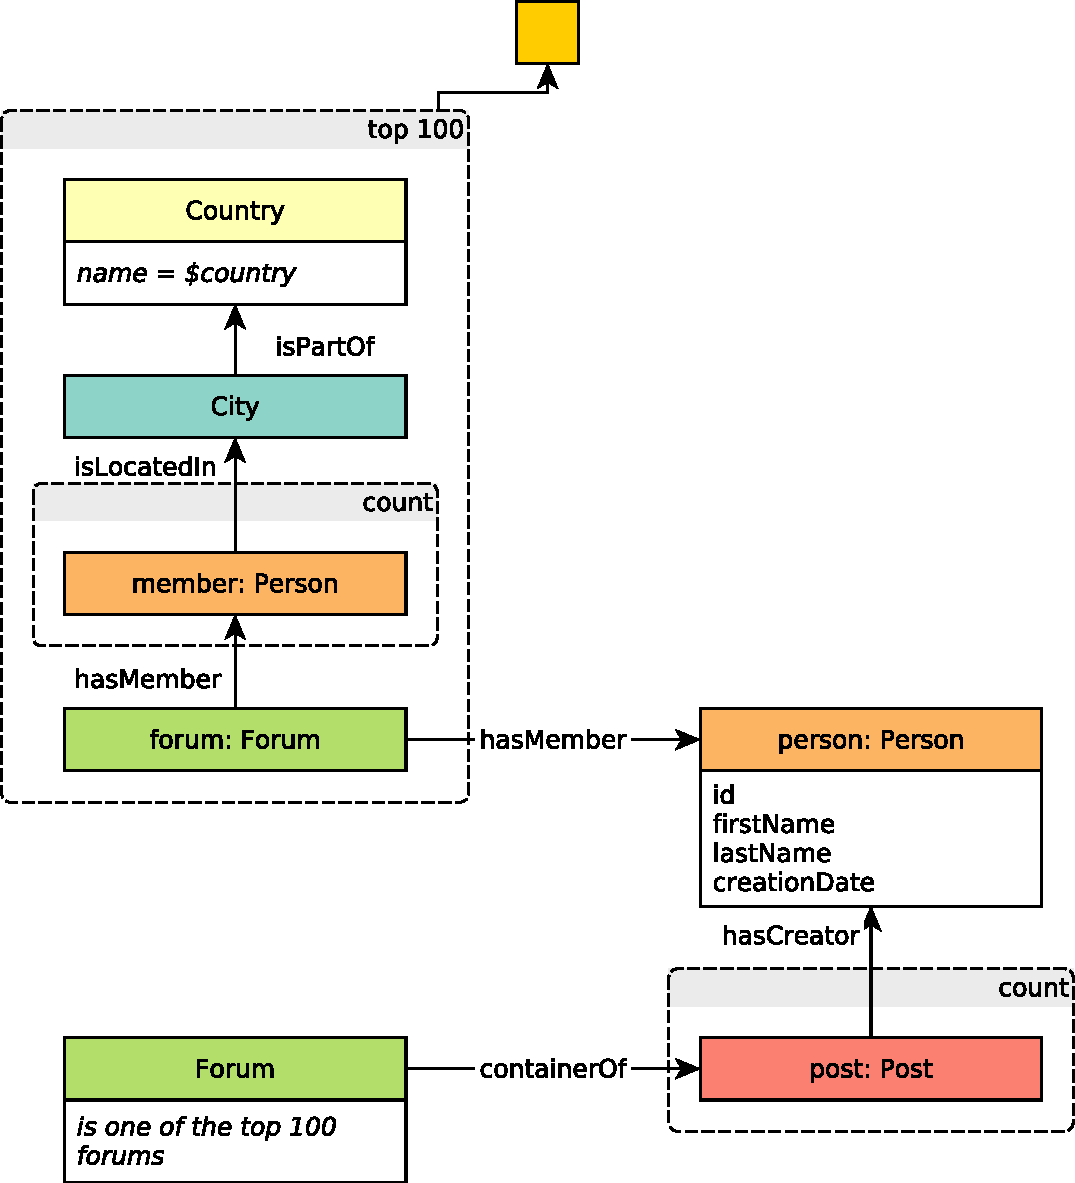
\includegraphics[scale=\patternscale,margin=0cm .2cm]{patterns/bi-read-05}\hfill\vadjust{} \\ \hline
%
	desc. & Find the most popular Forums for a given Country, where the popularity
of a Forum is measured by the number of members that Forum has from the
given Country.

For each member of the 100 most popular Forums, count the number of
Posts they made in any of those (most popular) Forums.
 \\ \hline
%
	
		params &
		\innerCardVSpace{\begin{tabularx}{\attributeCardWidth}{|>{\paramNumberCell}c|>{\varNameCell}M|>{\typeCell}m{\typeWidth}|Y|} \hline
		$\mathsf{1}$ & country
 & 32-bit Integer
 &  \\ \hline
		\end{tabularx}}\innerCardVSpace \\ \hline
	
%
	
		result &
		\innerCardVSpace{\begin{tabularx}{\attributeCardWidth}{|>{\resultNumberCell}c|>{\varNameCell}M|>{\typeCell}m{\typeWidth}|>{\resultOriginCell}c|Y|} \hline
		$\mathsf{1}$ & person.id
 & 64-bit Integer
 & R &
				 \\ \hline
		$\mathsf{2}$ & person.firstName
 & String
 & R &
				 \\ \hline
		$\mathsf{3}$ & person.lastName
 & String
 & R &
				 \\ \hline
		$\mathsf{4}$ & person.creationDate
 & DateTime
 & R &
				 \\ \hline
		$\mathsf{5}$ & postCount
 & 32-bit Integer
 & R &
				 \\ \hline
		\end{tabularx}}\innerCardVSpace \\ \hline
	
%
	
		sort		&
		\innerCardVSpace{\begin{tabular}{|>{\sortNumberCell}c|>{\varNameCell}l|>{\directionCell}c|} \hline
		$\mathsf{1}$ & postCount
 & $\desc
$ \\ \hline
		$\mathsf{2}$ & person.id
 & $\asc
$ \\ \hline
		\end{tabular}}\innerCardVSpace \\ \hline
	%
	limit & 100 \\ \hline
	%
	CPs &
	\multicolumn{1}{>{\raggedright}l|}{
		\chokePoint{1.2}, 
		\chokePoint{1.4}, 
		\chokePoint{1.5}, 
		\chokePoint{2.1}, 
		\chokePoint{2.2}, 
		\chokePoint{2.3}, 
		\chokePoint{2.4}, 
		\chokePoint{3.3}, 
		\chokePoint{5.3}, 
		\chokePoint{6.1}
		} \\ \hline
	%
	%
\end{tabularx}
\queryCardVSpace